\documentclass[11pt,a4paper]{article}
\usepackage[utf8]{inputenc}
\usepackage[spanish]{babel}
\usepackage{amsmath}
\usepackage{amsfonts}
\usepackage{amssymb}
\usepackage{graphicx}
\usepackage[left=2cm,right=2cm,top=2cm,bottom=2cm]{geometry}
\title{Universidad Politécnica de la Zona Metropolitana de Guadalajara}
\begin{document}

\maketitle

\begin{figure}[h]
\begin{center}

\includegraphics[scale=1]{1.jpeg}
\end{center}
\end{figure}


\begin{center}
\title{Amplificaciones con conexiones Darlington\\}
\author{Sistemas Electrónicos de Interfaz\\
Barrera Vazquez Omar\\
Ing. Mecatrónica 4B}
\end{center}


\newpage

\section{objetivo especifico de la practica}
Hacer el reemplazo de la utilización de transistores de baja capacidad, por transistores de potencia, demostrando la capacidad de utilización de los transistores Darlington en la electrónica de potencia.


\section{Materiales}

los materiales son sencillos de encontrar en tiendas de electrónica a un bajo costo, son los siguientes:

\begin{itemize}

\item 2 relevadores de 5V o 12V
\item 1 transistor de potencia tipo Darlington (preferente el TIP112)
\item 3 Leds de diferente color
\item 1 resistencia de 1K$\Omega$
\item 1 resistencia de 10K$\Omega$
\item 1 resistencia de 510$\Omega$
\item 3 resistencias de 220$\Omega$
\item 2 diodos rectificadores 1N4007
\item 4 colores diferente de cable para Protoboard
\item 1 LDR (fotoresistencia)
\item 1 opto-acoplador 4N25
\item 1 tarjeta arduino
\item 1 interruptor o push buttom
\item 1 relevador industrial de 24V
\item 1 fuente de alimentación con salidas a 5V y 12V (mínimo 3 salidas de cada uno)

\end{itemize}


\newpage

\section{qué es un Darlington?}

En anteriores practicas se trabajo con transistores de baja potencia como el \emph{transistor 2N2222} en cual nos servia como un interruptor controlado por un pulso eléctrico que provenía un microcontrolador (arduino para la practica) el cual activaba la base del transistor y este a su vez dejaba fluir la corriente para que el relevador junto con un indicador led era activado, en la actual practica se pretende activar algo que requiere mayor potencia, por lo que un transistor simple como lo es un \emph{2N2222} no soportara la potencia que producirá el consumo de corriente, por lo que se tiene una solución de simple uso en la electrónica de potencia.

Un Darlington es una configuración de dos transistores bipolares de tal modo que permite amplificar la potencia de salida con la que la corriente provoca. El Darlington trabaja de tal manera que la corriente entrara por los colectores de los transistores y uno enviara a través de su emisor la corriente a la base del segundo transistor, permitiendole amplificar la potencia de salida, se puede observar a mayor detalle en el siguiente diagrama de la figura 1:

\begin{figure}[hbtp]
\begin{center}
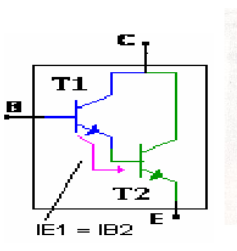
\includegraphics[scale=0.5]{1.png}
\caption{configuración eléctrica de un Darlington}
\end{center}
\end{figure}

Un tiempo atrás la construcción de un Darlington era con la unión de dos transistores físicos, tal como lo muestra la figura 1, este método se desarrollo por \emph{laboratorios Bell}, posteriormente el \emph{Ing. Darlington} desarrollo un encapsulado en el que en un solo dispositivo electrónico se podía encontrar esta configuración electrónica tal con lo muestra la figura 2:

\begin{figure}[h]
\begin{center}
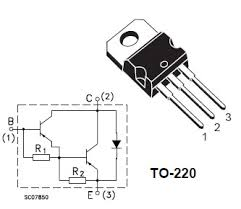
\includegraphics[scale=0.5]{2.png}
\caption{encapsulado actual de un transistor Darlington}
\end{center}
\end{figure}

El desarrollo de este tipo de transistor Darlington permitió el control de artefactos de potencia de hasta 3\emph{amperes} de corriente para controlar mecanismos como motores de bajo consumo, electrodomésticos y bombas de agua, ademas de mencionar su bajo costo y alta capacidad de resistir diferentes tipos de errores humanos, como cortos circuitos y altas tensiones.

\newpage

\section{Desarrollo de la practica}

Se comienza con el armado del circuito de la \emph{practica 2} que se puede observar el siguiente diagrama de la figura 3:

\begin{figure}[h]
\begin{center}
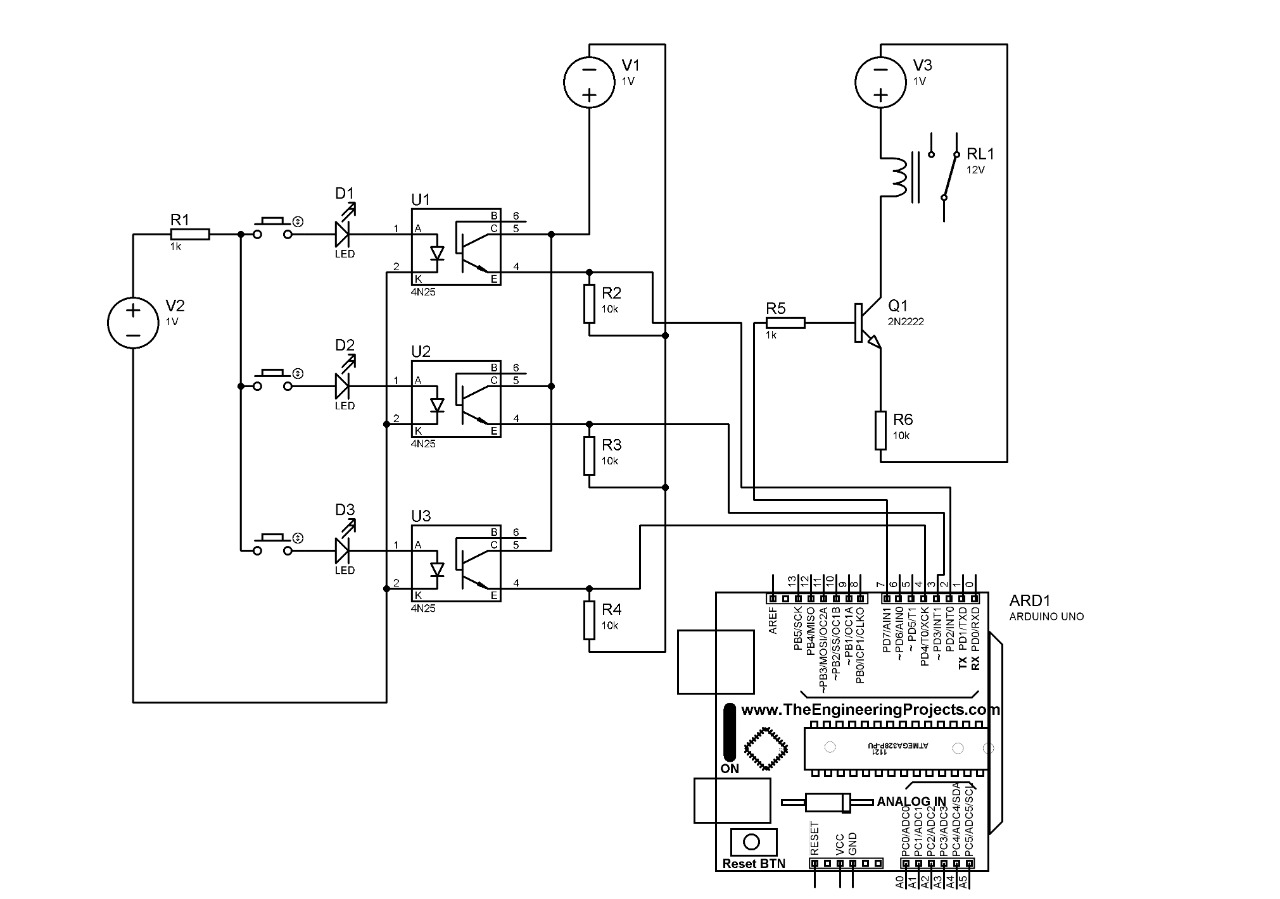
\includegraphics[scale=0.3]{2.jpeg}
\caption{diagrama eléctrico de la practica 2}
\end{center}
\end{figure}

El transistor Darlington sera intercambiado en lugar del transistor 2N2222 el cual se encuentra en la posición 2N2222, de tal manera que el Darlington haga la misma función pero con mas capacidad de tensiones y corrientes, en la practica se nos pide conectar un relevador de 24 volts en lugar del relevador de 12 volts, esto para comprobar que el Darlington funciona de la manera correcta, ya que el consumo de un relevador de 12v oscila en los 80\emph{miliamperios} en cambio el relevador industrial puede llegar a un consumo de 250\emph{miliamperios} en el cual se tiene una potencia de hasta 6\emph{watts}. La conexión en físico con un relevador industrial es la siguiente que se muestra en la figura 4:

\begin{figure}[h]
\begin{center}
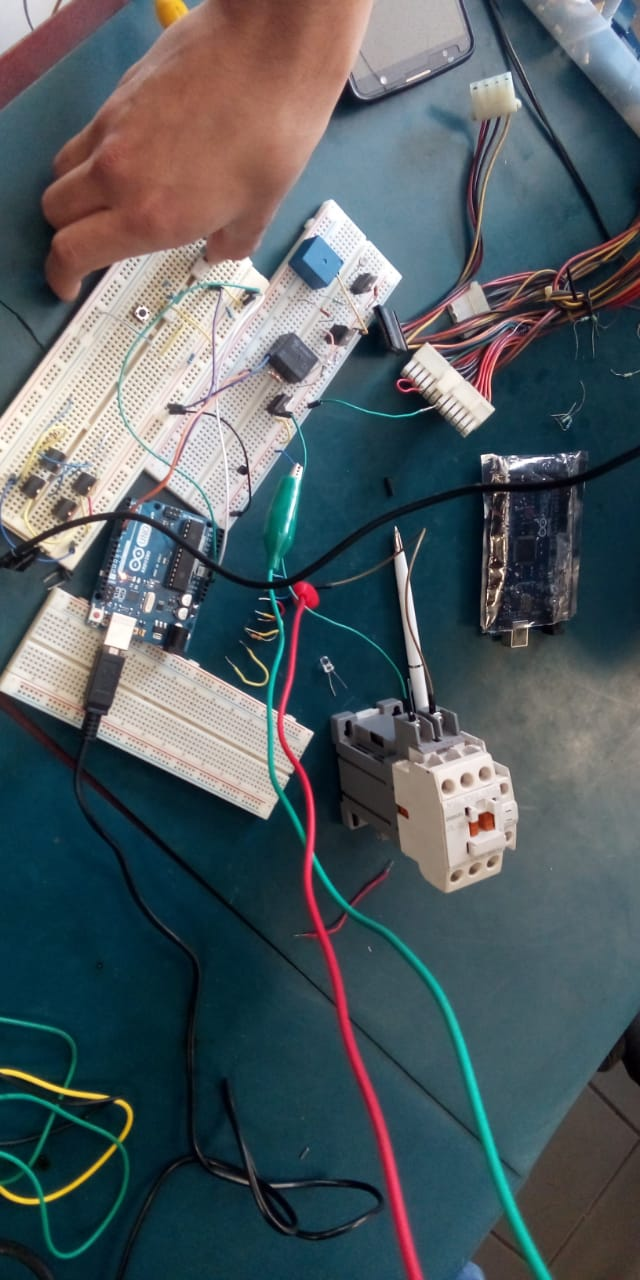
\includegraphics[scale=0.15]{3.jpeg}
\caption{conexión de relevador industrial}
\end{center}
\end{figure}

\newpage

De igual manera se puede trabajar con el diseño del Darlington, controlado con una LDR (fotoresistencia) la cual activara el relevador con la exposición al sol, el diagrama a utilizar puede ser como el mostrado en la figura 5:

\begin{figure}[h]
\begin{center}
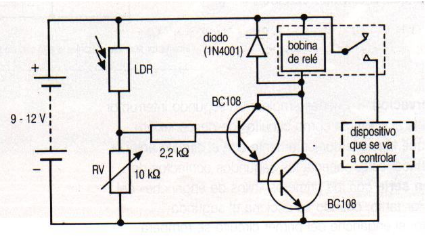
\includegraphics[scale=0.5]{4.png}
\caption{diagrama eléctrico de activación de relevador industrial con LDR}
\end{center}
\end{figure}

De esta forma se demuestra la capacidad de uso de un transistor Darlington el cual tiene una mayor resistencia a la potencia consumida a dispositivos conectados en sus terminales, su uso eleva la utilización en electrónica de potencia, para activar dispositivos con mayor consumo de tensión y corriente eléctrica.



-Datos y diagramas tomados de la siguiente referencia:\cite{morenoanalisis}

\bibliographystyle{apalike} 
\bibliography{ref.bib}

\end{document}